%------------------------------------------------------------------------------------
%	EDIT THIS BLOCK AS REQUESTED
%------------------------------------------------------------------------------------
\newcommand{\studentone}{[Your name]}			    % change to your name
\newcommand{\studentonenumber}{[XXXXXXXX]}		    % enter your student number 
% \newcommand{\studenttwo}{Steve Martin}			% change to your partner's name
% \newcommand{\studenttwonumber}{654321}			% enter your partner's student number
\title{Assignment 1}					            % change to the title of the experiment
% \author{\studentone and \studenttwo}				% you don't have to change this
\author{\studentone}	
\date{\today}										% this fills in today's date - don't change

%------------------------------------------------------------------------------------
%	SCROLL DOWN TO RESULTS AND ANALYSIS
%     You do not have to change anything in between!
%------------------------------------------------------------------------------------
\documentclass[12pt,oneside,oldfontcommands]{memoir}

%-----------------------------------------------------------------------------------
%	MARGIN AND HEADER/FOOTER SIZES
%------------------------------------------------------------------------------------
\setlrmarginsandblock{2.5cm}{2.5cm}{*}  		% left/right margins
\setulmarginsandblock{2.5cm}{2.5cm}{*} 			% top/bottom margins
\checkandfixthelayout							% checks the layout is correct
\setlength{\parindent}{0in}  					% no indent on start of paragraph
							
%-------------------------------------------------------------------------------------
%  PACKAGES
%-------------------------------------------------------------------------------------
\usepackage{amsmath,amsthm,amssymb,amsfonts}			% math fonts
\usepackage[english]{babel}								% hyphenation rules for english
\usepackage{graphicx}									% for importing pdf files 
\usepackage{siunitx}									% si units - extremely useful
\usepackage[usenames,dvipsnames,svgnames,table]{xcolor}	% defines the dvips color names
\usepackage{color,soul} 								% for highlight hi - hyphenation, underlining
\setulcolor{red} 										% set underline color
\setstcolor{green} 										% set overstriking color
\sethlcolor{green} 										% set highlighting color
\usepackage{fullpage,enumitem,amsmath,amssymb,graphicx}
%--------------------------------------------------------------------------------------------
%  GRAPHICS PATH
%--------------------------------------------------------------------------------------------
\graphicspath{{figures/}}								% put your figures in a folder called figures

%---------------------------------------------------------------------------
%  SOME NEW FUNCTIONS FOR IMPORTING FIGURES
%---------------------------------------------------------------------------
\newcommand{\placefigure}[1]{\centerline{\includegraphics[width=2 in]{#1}}} 
\newcommand{\placefigureandscale}[2]{\centerline{\includegraphics[width=#2 in]{#1}}} 

%-------------------------------------------------------------------------------------
%	TITLE PAGE MACRO
%------------------------------------------------------------------------------------
\makeatletter
\def\maketitle{%
  \null
  \thispagestyle{empty}
  \begin{center}\leavevmode
       \normalfont
       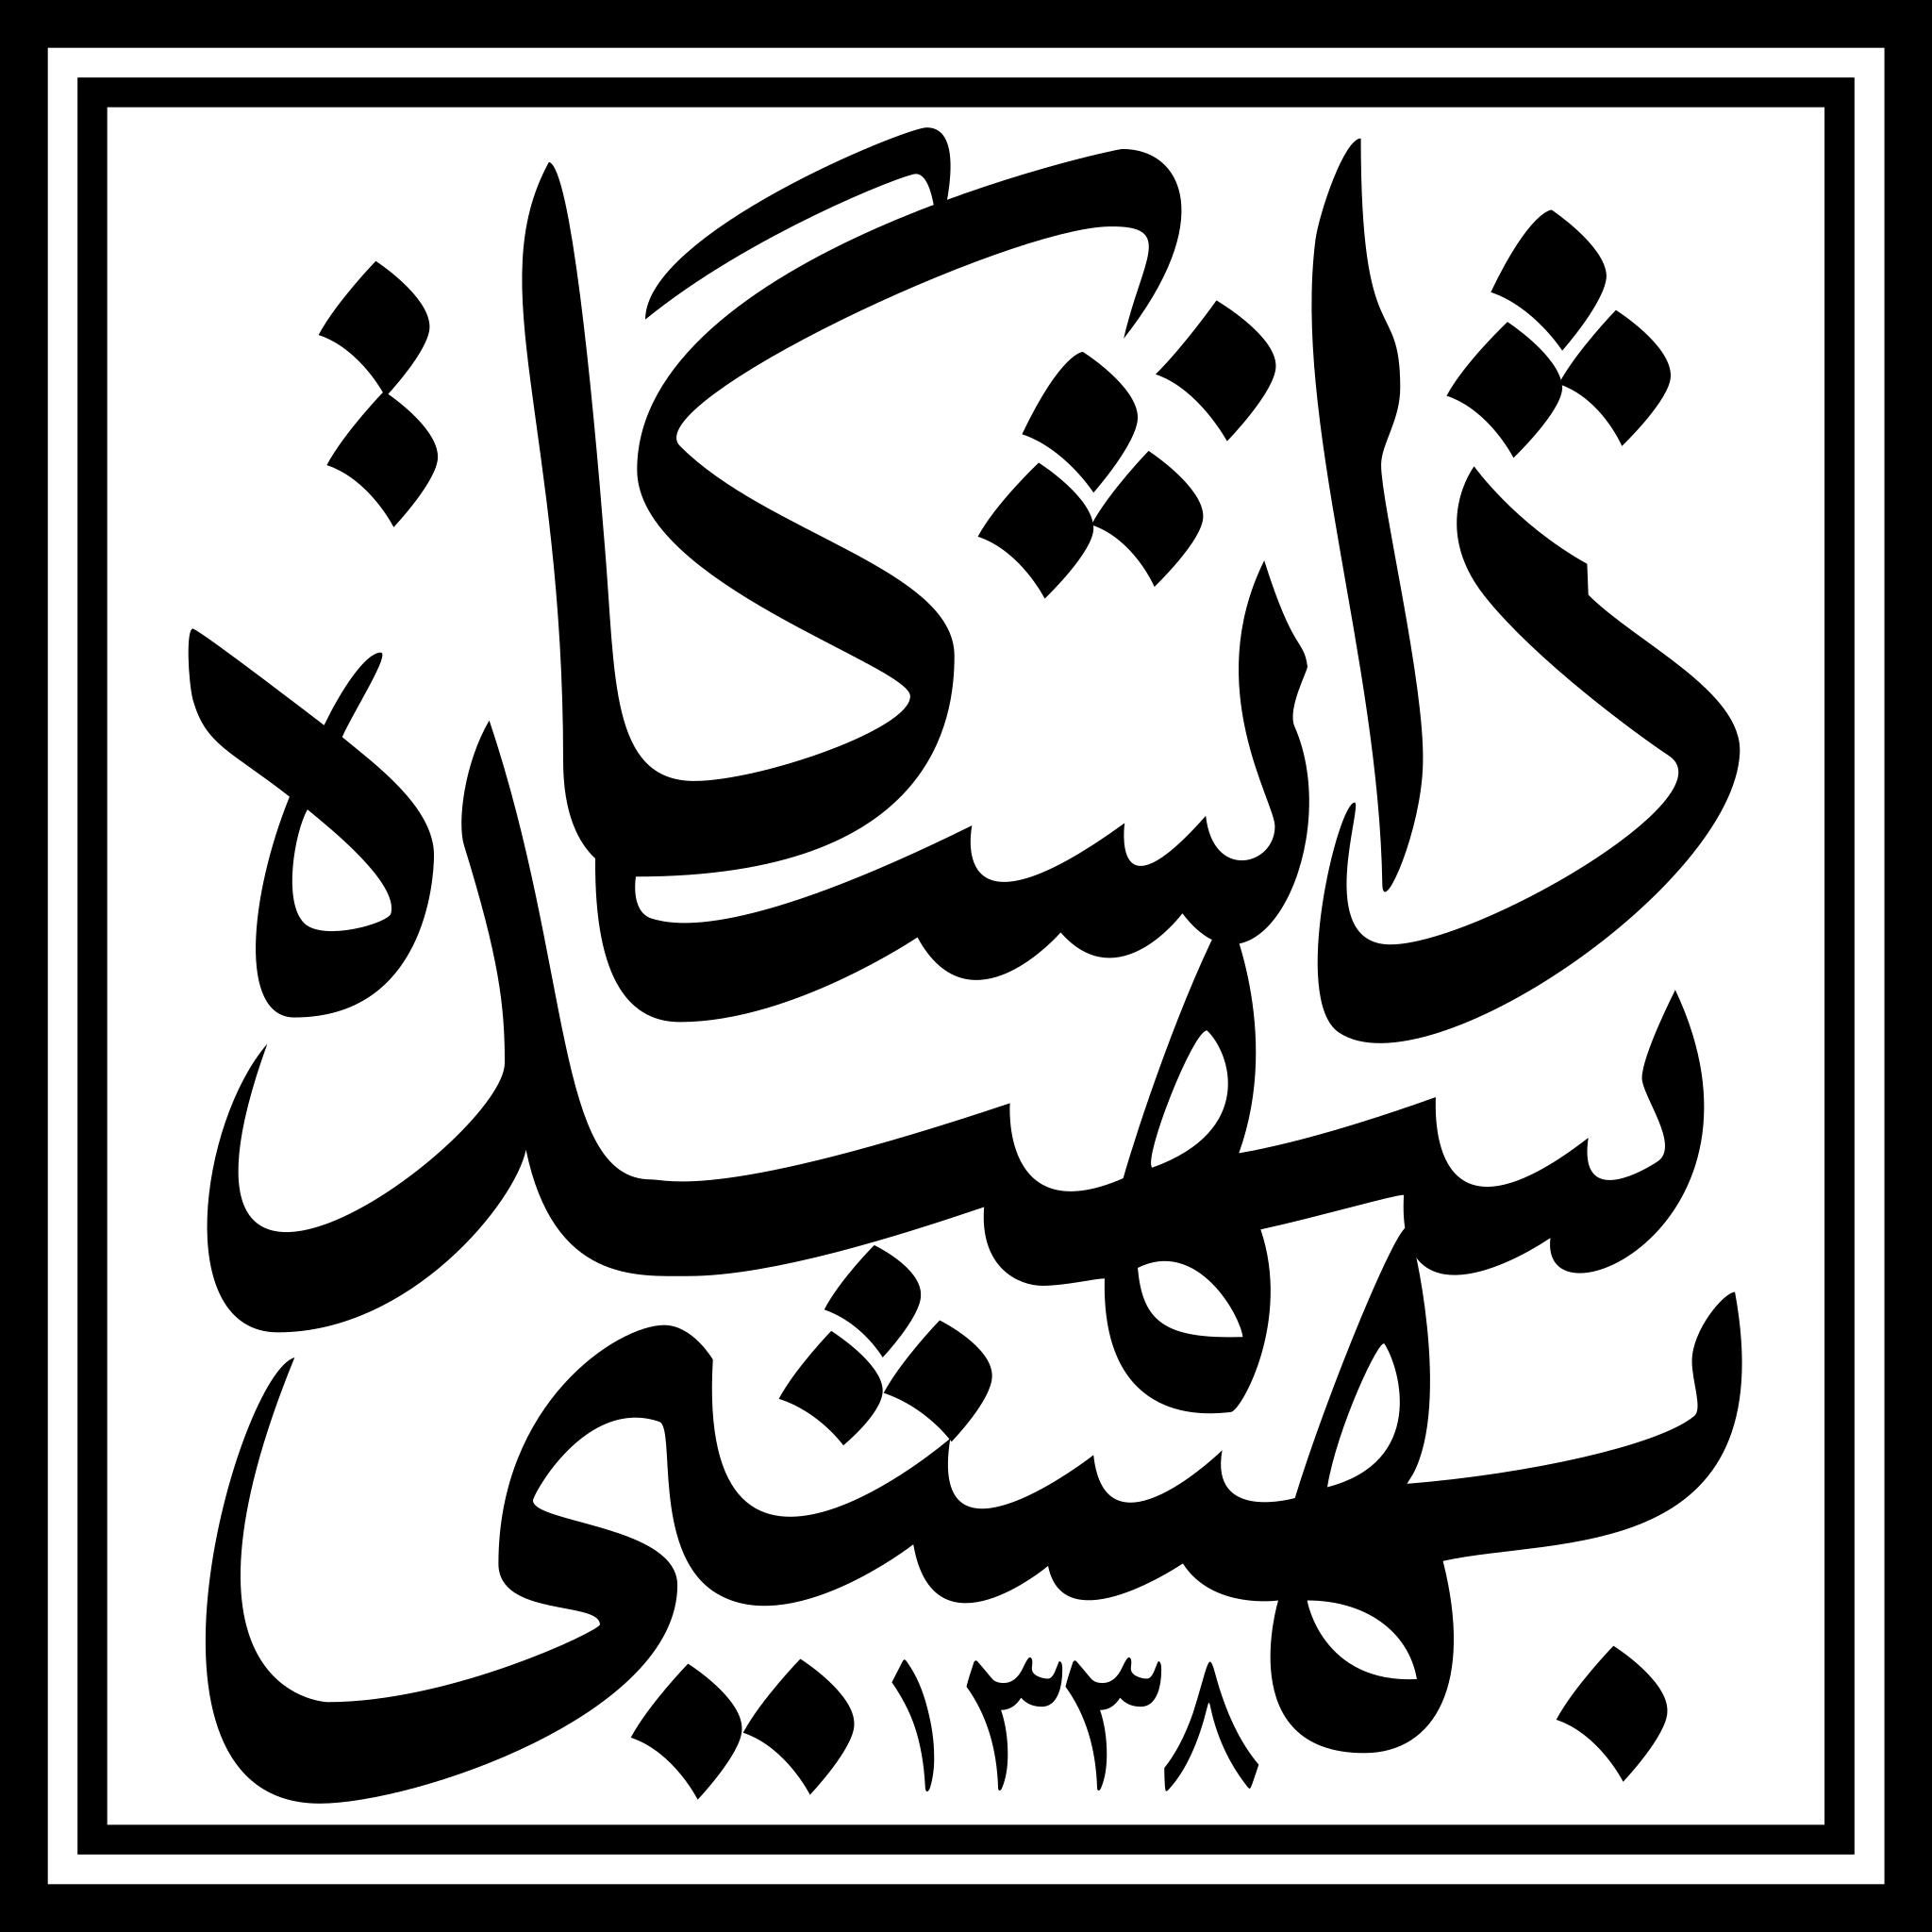
\includegraphics[width=0.3\columnwidth]{figures/Sbu-logo.svg.png}
       \vskip 0.5cm   
       \textsc{\Large Basics of cryptography (CE057)}\\[0.5 cm]
	     {\large \@date\par}
       \vskip 1.0cm
	\rule{\linewidth}{0.2 mm} \\[0.4 cm]
	{ \huge \bfseries \@title}\\
	\rule{\linewidth}{0.2 mm} \\[1.5 cm]
	
	\begin{minipage}{0.5\textwidth}
		\begin{flushleft} \large
			\emph{Name:} \studentone\\
			Student Number: \studentonenumber
			\end{flushleft}
			\end{minipage}~
			\begin{minipage}{0.4\textwidth}
			\begin{flushleft} \large
			% \emph{Partner:} \studenttwo\\
			% Student Number: \studenttwonumber
		\end{flushleft}
	\end{minipage}\\[2 cm]
   \end{center}
   \vfill
   \null
   \cleardoublepage
  }
\makeatother

%-------------------------------------------------------------------------------------------
%	START OF DOCUMENT
%--------------------------------------------------------------------------------------------
\begin{document}
  \maketitle
  \begin{center}

  \vspace{-0.3in}
  \begin{tabular}{rl}
  % Collaborators: & 
  \end{tabular}
  \end{center}
    \textbf{Due date: 1 March 2023, 23:59 (GMT+3:30)}\\
    In this assignment you are going to answer questions related to historical ciphers
    and information theory.
    \begin{itemize}
        \item By turning in this assignment, I declare that all of this is my own work.
        \item This is an individual assignment. Please mention your name and student number in
        submission. You have to hand in a  \textbf{SINGLE} document (PDF) with your answers
        and your source code (if any).\textbf{ Also, be aware that any form of plagiarism
        will not be condoned.}
        \item Your code must be written in C, Java, Python or Golang, although we encourage you to use Python for simplicity.
        \item Pose your questions on the Telegram group, so that your fellow students can also
        read them.
        \item \textbf{Explain and motivate all your answers!}
    \end{itemize}

  \noindent
  \rule{\linewidth}{0.4pt}
%--------------------------------------------------------------------------------------------
%	Section
%--------------------------------------------------------------------------------------------
  \section*{Introduction to Cryptography (24 points)}

  \begin{enumerate}[label=(\alph*)]
    \item Consider a group of 20 persons who want to use symmetric-key cryptography to create pair-wise secure communications.How many keys need to be exchanged in total?https://www.overleaf.com/project/63e8ba13f1e8c0d77c622557
    \item You will consider the relation between passwords and key size. For this purpose
    we consider a cryptosystem where the user enters a key in the form of a password.\\
    1. Assume a password consisting of 8 letters, where each letter is encoded by the
    ASCII scheme (7 bits per character, i.e., 128 possible characters). What is the
    size of the key space which can be constructed by such passwords?\\
    2. What is the corresponding key length in bits?\\
    3. Assume that most users use only the 26 lowercase letters from the alphabet instead of the full 7 bits of the ASCII-encoding. What is the corresponding key length in bits in this case?\\
    4. At least how many characters are required for a password in order to generate a
    key length of 128 bits in case of letters consisting of\\
    a. 7-bit characters?\\
    b. 26 lowercase letters from the alphabet?
  \end{enumerate}

%--------------------------------------------------------------------------------------------
%	Section
%--------------------------------------------------------------------------------------------
  \section*{Classical Systems - Decrypt (46 points)}
    In this exercise, you are given several ciphertexts originating from classical systems. For each ciphertext, you need to answer the following questions:
    \begin{itemize}
        \item Which encryption scheme was used?
        \item What was the original plaintext message?
        \item What was the encryption key?
    \end{itemize}
    Or explain why it is not possible to decipher it.
  \begin{enumerate}[label=(\alph*)]
    \item Consider the ciphertext:\\
        "ZRPHQ, OLIH, DQG IUHHGRP!"
    \item Consider the ciphertext:\\
        ”JOVJVSHAL DHZ PUCLUALK MVBY AOVBZHUK FLHYZ HNV PU HZTHSS CPSSHNL PU OVUKBYHZ HUK OHZ AOYPCLK LCLY ZPUJL”
    \item Consider the ciphertext:\\
        The ciphertext is available in "permutation cipher.txt"
    \item Find the key for the following Vigenère-ciphertext and explain your approach.\\
    \textbf{Hint: }You should subtract 1 from the estimator of the keylength you obtained from this ciphertext.\\
    The ciphertext is available in "vigenère cipher.txt"

    \item Hill cipher is a polygraphic substitution cipher based on linear algebra. Using this algorithm we encrypt plain text see in below. Let's guess the key.\\
    Plain text = [5 17, 8 3]\\
    Cypher text = [15 16, 2 5]
    
  \end{enumerate}
%--------------------------------------------------------------------------------------------
%	Section
%--------------------------------------------------------------------------------------------
  \section*{Classical Systems - Encrypt (30 points)}

  \begin{enumerate}[label=(\alph*)]
    \item Encrypt the given plain text using mentioned algorithms and key. (please ignore the white space)\\
    plain text = This is a secret message.
    \begin{itemize}
        \item Shift cipher algorithm, k = 8
        \item Affine cipher algorithm, k = (5, 21). Is it possible to encrypt this plain text using this algorithm? explain.
        \item Playfair cipher
        \item Vigenere cipher, k = (8, 2, 10, 7, 25, 6)
    \end{itemize}
    
  \end{enumerate}

\end{document}